\documentclass{report}

% depricated
\title{
	\iffalse
	\begin{tikzpicture}[remember picture,overlay]
		\node[anchor=north west,yshift=-5pt,xshift=-200pt]%
		at (current page.north east)
		{
\includegraphics[height=30mm]{unitn-logo}};
	\end{tikzpicture}
	\huge 
	\fi
	FixMi \\
	Analisi dei Requisiti
}
\author{Giovanni Santini, Riginel Ungureanu, Valerio Asaro}
\date{Anno accademico 2023/2024}

% for the image in the title
\usepackage{tikz}

% custom spacing
\usepackage{setspace}
\onehalfspacing

% footer and header
\usepackage{fancyhdr}
% \setlength{\headheight}{15.2pt}

% Table of contents link to corresponding sections
\usepackage{hyperref}
\hypersetup{
	colorlinks,
	citecolor=black,
	filecolor=black,
	linkcolor=black,
	urlcolor=black
}

% Remove che "Chapter" string before chapters
\iffalse
\makeatletter
\def\@makechapterhead#1{%
	\vspace*{50\p@}%
	{\parindent \z@ \raggedright \normalfont
		\interlinepenalty\@M
		\Huge\bfseries  \thechapter.\quad #1\par\nobreak
		\vskip 40\p@
}}
\makeatother
\fi

% Fancy chapters
\usepackage[Bjarne]{fncychap}
% options: Sonny, Lenny, Glenn, Conny, Rejne, Bjarne, Bjornstrup

%glossario
% \usepackage{glossaries}

\begin{document}


%title page
\begin{titlepage}
	\begin{figure}[t]
		\centering
\includegraphics[width=0.3\textwidth]{unitn-logo}
	\end{figure}
	\begin{center}
		\textsc{ \LARGE{Università degli Studi di Trento \\}}
		\textsc{ \LARGE{Facoltà di Informatica\\ }}
		\textnormal{ \LARGE{Corso di Ingegneria del Software\\}}
		\vspace{30mm}
		\fontsize{10mm}{7mm}\selectfont 
		\textup{FixMi \\ Analisi dei Requisiti}\\
	\end{center}
	
	\vspace{25mm}
	
	\centering
	\large Giovanni Santini\\ Riginel Ungureanu \\ Valerio Asaro
	
	\vspace{20mm}
	
	\centering{\large{Anno Accademico 2023/2024 \\ Trento }}
	
\end{titlepage}


% use header and footers
\pagestyle{fancy}
\fancyhead[R]{\chaptername\ \thechapter}  % header

%\maketitle
\tableofcontents
\newpage





\section{Scopo del documento}
Il seguente documento riporta la definizione e l'analisi del progetto "FixMi" in linguaggio naturale.
In particolare il documento mira a:

\begin{enumerate}
		
	\item Stabilire gli obiettivi del progetto.
	\item Definire i requisiti funzionali e non funzionali.
	\item Presentare i requisiti di Front-End del progetto.
	\item Presentare i requisiti di Back-End del progetto.
	\item Stabilire ruoli e funzioni dei singoli membri del team di sviluppo.
	\item Definire tecniche e strumenti utili alla realizzazione del progetto.

\end{enumerate}


\section{Informazioni del Documento}

% table
\begin{center} % center the table
	\centering
	\begin{tabular}{ |p{4cm}|p{4cm}|  }
		\hline
		\centering Campo & \qquad\qquad Valore \\ % I found no other way...
		\hline
		Titolo del Documento & Analisi dei Requisiti \\
		\hline
		Titolo del Progetto & FixMi \\
		\hline
		Autori del Documento &
		Giovanni Santini \\ & Riginel Ungureanu \\ & Valerio Asaro \\
		\hline
		Responsabile del Progetto & Riginel Ungureanu\\
		\hline
		Versione del documento & 1.1 \\
		\hline
	\end{tabular}
\end{center}


\chapter{Obiettivo del progetto}


Di seguito vengono illustrati in maniera discorsiva gli obiettivi principali e secondari del progetto in questione.

\section{Obiettivo Principale}

L’obiettivo del progetto è la realizzazione di una Web-App denominata "Fix Mi": un'applicazione web gestionale sviluppata per un negozio di articoli informatici ed elettronici “retrò”. Tale software svolgerà il ruolo di supporto all’attività di commercio e riparazione dei dispositivi elettronici mettendo in comunicazione datore di lavoro, dipendenti e clienti.


\section{Obiettivi Secondari}

Successivamente vengono elencati gli obiettivi secondari del progetto, numerati tramite acronimo OSx (Obiettivi Secondari), dove x è il numero che identifica inequivocabilmente un obiettivo da un altro. Questi obiettivi estendono quello principale e non sono da considerare di minore importanza durante l’analisi dei requisiti.


\subsection*{OS1 Autenticazione}
L’applicazione dispone di un sistema di distinzione dei ruoli Manager, Dipendenti e Clienti. Tale sistema permetterà diverse funzionalità in base al livello di autorizzazione.



\subsection*{OS2 Magazzino}
Il sito presenta ai dipendenti e al manager un sistema di gestione del magazzino con il quale si potrà aggiungere e rimuovere merce, oltre a controllarne la disponibilità.


\subsection*{OS3 Negozio}
Il sito offre ai clienti uno shop, con catalogo interfacciato con il magazzino, che permette loro di effettuare acquisti. I dipendenti potranno vedere gli ordini e le richieste di vendita in modo da gestirle.


\subsection*{OS4 Riparazione}
L’applicazione permette ai clienti di richiedere la riparazione di un proprio articolo ed organizzare l’attività di riparazione di tale articolo tra i dipendenti.


\subsection*{OS5 Assistenza}
Il sito presenta ai clienti la lista dei contatti dell’azienda, nonché la possibilità di inserire una richiesta di assistenza relativa al sito, un ordine, o una riparazione. I dipendenti potranno gestire le richieste e comunicare direttamente con i clienti.


\subsection*{OS6 Feedback}
Gli utenti potranno inviare feedback sulla qualità del servizio offertogli.

\subsection*{OS7 Gestione Dipendenti}

Il manager può gestire i profili dei dipendenti. Ciò include l’aggiunta di un nuovo profilo, la rimozione o la modifica. Il sito inoltre permette di vedere le statistiche dei dipendenti.


\subsection*{OS8 Gestione Task}
L’applicazione presenta ai dipendenti e al manager un sistema di gestione delle varie tipologie di task, ossia le varie attività che i dipendenti devono svolgere, assegnando ad ogni dipendente delle task appropriate alle proprie abilità.


\chapter{Requisiti}
Posto l’obiettivo del progetto segue la definizione dei requisiti del sistema, suddivisi in Requisiti Funzionali (RF) e Requisiti Non Funzionali (RNF).



\section{Requisiti Funzionali}
Segue la lista dei Requisiti Funzionali (RF) individuati per il progetto.


\subsection*{RF0 Requisiti Generali}
Il sito deve manifestare una distinzione esplicita tra i tre tipi di utente, ossia Cliente, Dipendente e Manager, ognuno con accesso a funzionalità e privilegi diversi.
In vista di questo, la seguente sezione verrà divisa in base al tipo di utente interessato.

\subsection{Utente Non Autenticato}

\subsection*{RF1 login}
Il sito deve presentare una pagina di login:
\begin{enumerate}
	\item La pagina richiede due campi “email” e “password” associati ad un profilo per identificarsi ed accedere alle varie funzionalità dell’applicazione in base al proprio livello di autorizzazione (Manager, Dipendente, Cliente) specificate più avanti.
	
	\item L'utente verrà autenticato se e solo se i campi "email" e "password" corrispondono entrambi ad un profilo già registrato nel sistema.
	
	\item Nel caso il login fallisse, ossia la email o la password non corrispondessero ad un utente registrato, l’applicazione mostrerà una nuova pagina di login.
	
	\item L’utente deve essere in grado di raggiungere la pagina di registrazione specificata in RF2 in qualsiasi momento dalla pagina di login.
	
\end{enumerate}

	\subsubsection{RF1.2 2FA}
	La pagina di login deve implementare una tecnologia 2FA (Two Factor Authentication) secondo le seguinti modalità:
	
	\begin{enumerate}
	\item L’utente dovrà inserire un codice OTP (One-Time Password), generato sul momento e ottenuto attraverso la propria email, prima di completare ogni accesso all’applicazione. 
	
	\item 	L’autenticazione non potrà procedere finché l’utente non avrà inserito il corretto codice OTP.
	
	\item L’utente avrà sempre la possibilità di ricevere un nuovo OTP tramite email, il codice precedente non sarà più valido per effettuare l’autenticazione.

	\end{enumerate}
	
\subsubsection*{RF1.3 Cambio Password}
Il sito deve offrire la possibilità all’utente di cambiare password:
	\begin{enumerate}
		\item L'applicazione deve inviare un link all'utente attraverso email che porterà ad una nuova pagina. La pagina presenterà un campo "nuova password".
		
		\item La nuova password dovrà essere digitata due volte per ridurre la probabilità di errori di battitura.
		
		\item La nuova password deve rispettare i vincoli specificati in RF2.
		
		\item Qualora non vi fosse alcun profilo associato alla la mail inserita, il processo fallirà e verrà caricata la pagina di login.
	\end{enumerate}


\subsection*{RF2 Registrazione}
Il sito deve dare la possibilità ad un utente di registrarsi:
\begin{enumerate}
	\item La pagina presenta i campi "email", "password" (due volte), "username" e "nazionalità". 
	\item La password deve essere conforme come specificato in RNF3.
	\item La nazionalità deve essere scelta da una lista finita di nazioni disponibili.
\end{enumerate}

\subsubsection*{RF2.1 Verifica Email}
Per terminare la registrazione con successo, l'applicazione deve verificare la mail dell'utente

\begin{enumerate}
	\item L'applicazione deve inviare un codice di 6 cifre, generato randomicamente sul momento, alla email specificata dall’utente e mostrare un campo "inserisci codice".
		
	\item L’utente avrà sempre la possibilità di inviare un nuovo codice di verifica del profilo. Il codice precedente non sarà più valido per completare la registrazione.
		
\end{enumerate}


\subsubsection*{RF2.2 Terminazione Registrazione}
\begin{enumerate}
	\item Qualora il codice inserito nel campo "inserisci codice" corrispondesse a quello inviato tramite email, e i campi "email" e "password" fossero validi, la registrazione terminerà con successo e l'applicazione caricherà automaticamente la pagina di login (RF1).
	\item Se una delle condizioni del punto precedente non venisse soddisfatta, la registrazione non proseguirà e la pagina permetterà di effettuare modifiche ai dati inseriti nei campi
	\item Il livello di permessi del nuovo profilo successivamente alla registrazione è di tipo Cliente.
	\item La registrazione non deve terminare con successo se un utente tenta di registrarsi con una email a cui è associato un profilo esistente.

\end{enumerate}


\subsection*{RF3 Negozio}
Il sito presenta all’utente non autenticato una pagina "Negozio”: 

\begin{enumerate}
	\item La pagina permette di visualizzare gli oggeti presenti nel magazzino al momento del caricamento della stessa
	
	\item L’utente deve essere in grado di ordinare gli oggetti per nome o per prezzo tramite un bottone, ricercare una stringa tra tutti gli oggetti nel magazzino tramite una barra di ricerca.
	
	\item Ogni oggetto deve avere una pagina dedicata accessibile tramite un click sull’oggetto
\end{enumerate}


\subsection*{RF4 About / Contatti}
L’applicazione deve offrire all’utente una pagina dove sono visibili dati utili riguardo l'azienda:

\begin{enumerate}
	\item Descrizione dell'azienda.
	\item Una lista contenente varie Frequently Asked Questions (FAQ) riguardo il funzionamento del sito.
	\item Contatti dell’impresa: numeri di telefono, email e indirizzo.
	\item Il sito deve mostrare inoltre un riquadro con una mappa dove è possibile visualizzare la posizione del negozio.
\end{enumerate}


\subsection{Cliente}
Il sito deve dare la possibilità al cliente di autenticarsi attraverso la pagina di login come specificato in RF1 inserendo le proprie credenziali (email e password) inserite in fase di registrazione, in modo da poter accedere alle funzionalità elencate di seguito:

\subsection*{RF5 Negozio}
Il sito deve permettere al cliente, oltre alle funzionalità definite in RF3 per gli utenti non autenticati, le seguenti funzionalità:

\subsubsection{RF5.1 Carrello}
Il sito deve avere una pagina dedicata al carrello del cliente.
Il sito deve permettere al cliente autenticato, nella pagina dedicata a un specifico articolo, di inserirlo nel proprio carrello attraverso un pulsante.

\begin{enumerate}
	\item La pagina deve avere un elenco di tutti i prodotti che sono stati immessi nel carrello. Ogni prodotto nell’elenco deve  avere il nome, il prezzo, una foto e  un pulsante “rimuovi”
	
	\item La pagina deve permettere al cliente di rimuovere un elemento dal proprio carrello premendo il pulsante “rimuovi” dell’elemento.

	\item Ogni prodotto deve portare alla pagina dedicata allo stesso cliccando sul nome nell’elenco.
	
	\item La pagina deve mostrare il prezzo totale, ossia la somma dei prezzi degli elementi del carrello.

	\item La pagina deve avere un tasto “procedi al pagamento” con il quale si procede alla pagina di pagamento specificata sotto.

\end{enumerate}

\subsubsection*{RF5.2 Pagamento}
La pagina deve fornire diversi metodi di pagamento:

\begin{enumerate}
	\item La pagina deve fornire il pagamento con bancomat interfacciandosi con la banca dell'azienda
	\item La pagina deve fornire il pagamento tramite Paypal interfacciandosi al sito stesso.
	\item Una volta effettuato il pagamento con successo, il sito deve fornire un riepilogo dell’acquisto e un messaggio che invita il cliente a recarsi in negozio per il ritiro dei prodotti.
	\item Il sito deve creare per i dipendenti una task “magazzino” (RF9), dettagliando i prodotti richiesti.
	\item Il sito deve inviare i dettagli del pagamento al software di accounting scelto.
	\item Il sito deve svuotare gli elementi del carrello dell’utente una volta effettuato il pagamento.
\end{enumerate}

\subsection*{RF6 Riparazione}

Il sito deve offrire al cliente la possibilità di inviare, attraverso un'apposito form, una richiesta di riparazione per un proprio articolo di elettronica.
\begin{enumerate}

	
	\item Il form ha i campi "nome", "cognome", "email", "numero di telefono", "descrizione del problema", "foto" e un bottone "Invia".
	
	\item Successivamente all’invio della richiesta da parte del cliente, l’applicazione deve generare una task di tipo “riparazione”. Il sistema di task è specificato in RF9
	
	\item Qualora il cliente abbia inviato una riparazione, il sito deve mostrare al cliente lo stato della propria riparazione in un'apposita pagina "stato riparazioni", interfacciandosi con il sistema di task specificato in RF9.
	
\end{enumerate}

\subsection*{RF7 Assistenza}
Il sito deve permettere al cliente di richiedere assistenza e comunicare con l'azienda attraverso un form:

\begin{enumerate}
	\item Il form ha i campi "email", "descrizione richiesta" e un bottone "Invia".
	
	\item Successivamente all’invio della richiesta di assistenza da parte del cliente, l’applicazione deve generare una task di tipo “assistenza”. Il sistema di task è specificato in RF9.
	
	
\end{enumerate}

\subsection*{RF8 Feedback}
Il sito deve dare la possibilità al cliente di inviare anonimamente del feedback attraverso una pagina dedicata.
\begin{enumerate}
	\item La pagina contiene i campi "disponibilità azienda", "velocità riparazione", "soddisfazione riparazione", "soddisfazione sito web", "idee per migliorare" e un bottone "Invia".
	
	\item Il sito deve implementare un sistema per evitare lo spam da parte dei soggetti maliziosi, oltre che un filtro  per le profanità.
	
\end{enumerate}

\subsection{Dipendente}
Il sito deve dare la possibilità al dipendente di autenticarsi attraverso la pagina di login (RF1) inserendo le proprie credenziali (email e password) fornitegli dal manager, in modo da poter accedere alle funzionalità riservate ai dipendenti elencate qui sotto.

\subsection*{Il Sistema Task}
Il sistema delle task è centrale alla gestione dell'attività aziendale e al funzionamento dell'applicazione. In seguito vi è una descrizione del suo funzionamento

\subsubsection*{Definizione Task e Task-tag}
Una task è un'attività sulla quale un dipendente o un manager può decidere di lavorare. Esistono diverse tipologie di task, caratterizzate da una \textit{task-tag}. \\
Una \textit{task-tag} è una e una sola stringa tra le seguenti:
\begin{itemize}
	\item Magazzino
	\item Negozio
	\item Assistenza e Supporto
	\item Riparazione
\end{itemize}
Le tasks possono essere in uno dei seguenti stati: 
\begin{itemize}
	\item Da eseguire
	\item In lavorazione
	\item In pausa
	\item Completata
	\item Fallita
\end{itemize}

\subsubsection*{Descrizione delle singole tasks}

In seguito vi è una descrizione del contenuto di ogni tipologia di task:


\begin{enumerate}
	\item Magazzino: il dipendente può visualizzare, aggiungere o rimuovere oggetti dal magazzino.
	
	\item Negozio: il dipendente può accedere al sistema di contabilità per aggiornare eventuali entrate / uscite del negozio. Il dipendente ha anche accesso al magazzino come nel punto precedente.
	
	\item Assistenza: il dipendente visualizza la richiesta di supporto dal cliente, la descrizione della richiesta, la email del cliente ed eventuali altri dati inseriti dal cliente. Il dipendente potrà rispondere per mail al cliente in base alle esigenze del caso, secondo la propria discrezione.
	
	\item Riparazione: il dipendente potrà prendersi carico di una riparazione selezionando e avviando la task. Qualora ci fossero problemi e/o ritardi, il dipendente potrà mettere la task in pausa e riprenderla in qualsiasi momento. Una volta che la riparazione viene terminata, il dipendente segnerà la task come completata o fallita nel caso la riparazione non avesse successo.
	
\end{enumerate}

\subsection*{Definizione work-tag}
Ad ogni profilo dipendente sono associate una o più \textit{work-tag}. Una \textit{work-tag} è una stringa dello stesso tipo di una \textit{task-tag} (Magazzino, Negozio, Assistenza, Riparazione).\\
Ogni dipendente potrà lavorare solo sulle task che hanno gli stessi o meno \textit{task-tag} rispetto ai \textit{work-tag} del dipendente.


\subsection*{RF9 Pagina Task}

Il sito deve offrire una pagina “Task” ai dipendenti autenticati:

\begin{enumerate}
	\item La pagina permetterà al dipendente di visualizzare una lista di task e i corrispettivi \textit{task-tag}.
	
	\item Le task visualizzate sono automaticamente selezionate per il dipendente autenticato dall’applicazione in base ai \textit{work-tag} associati al proprio profilo
	
	\item Le task visualizzate sono solo quelle con lo stato "Da eseguire" oppure "In pausa"

	
\end{enumerate}

\subsubsection*{RF9.1 Interagire con le tasks}

Nella pagina task, il dipendente deve essere in grado di:


\begin{enumerate}
	\item Selezionare una task dalla lista da eseguire o da quelle messe in pausa, contrassegnandola come in lavorazione, solo nel caso in cui il dipendente non presenti alcuna task in lavorazione.
	
	\item Mettere in pausa la task in esecuzione, la task verrà contrassegnata come “In pausa” e il dipendente potrà selezionare una nuova task dalla lista.
	
	\item Contrassegnare una task come “completata” e salvarla in una lista di task completate, insieme al nome del / dei dipendente/i responsabili del completamente e alla data, oppure come “fallita” nel caso ci fossero stati dei problemi. Il dipendente allora potrà scegliere una nuova task dalla lista.
\end{enumerate}

\subsection{Manager}
Il sito deve dare la possibilità di autenticazione del manager nella pagina di login, fornendo email e password del profilo manager.

\subsection*{RF10}
Se un profilo è di tipo manager, deve poter accedere a tutte le funzionalità del profilo “dipendente” specificate sopra. In aggiunta il manager deve essere in grado di:

\subsubsection*{RF10.1 Gestione dei Dipendenti}
Il manager deve essere in grado di:

\begin{enumerate}
	
	\item Aggiungere profili “dipendente” dall’applicazione inserendo l’email del profilo in un apposito campo
	\item Aggiungere dati Anagrafici associati all'account dipendente , "nome", "cognome", "data di nascita", "giorno assunzione".
	\item Rimuovere dipendenti tramite un bottone che permette di selezionare la 
	email del dipendente e rimuoverla dalla lista dipendenti.
	
	\item Assegnare e rimuovere una o più \textit{work-tag} ai dipendenti. 
	
	\item Visualizzare informazioni dei dipendenti in apposita pagina, in particolare:
	
	\begin{itemize}
		\item Informazioni Biografiche.
		\item Storico con attività e record delle task svolte / in svolgimento. Lo storico deve poter essere filtrato e ordinato tramite data di inizio e fine task, nome dipendente, lista di task-tag.
		
	\end{itemize}
	
	\item Il profilo manager ha tutte le \textit{work-tag} assegnate per il proprio profilo.
		
\end{enumerate}


% table, da updateare
\begin{table}[h]
\begin{center} % center the table
	\centering
	\begin{tabular}{ |p{4cm}|p{4cm}|  }
		\hline
		\centering Obiettivi & \qquad\qquad Requisiti \\ % I found no other way...
		\hline
		OS1 Autenticazione & RF1, RF2 \\
		\hline
		OS2 Magazzino & RF9 \\
		\hline
		OS3 Negozio &
		RF3, RF9 \\
		\hline
		OS4 Riparazione & RF6, RF9\\
		\hline
		OS5 Assistenza & RF7, RF9 \\
		\hline
		OS6 Feedback & RF8, RF9 \\
		\hline
		OS7 Gestione dei Dipendenti & RF10 \\
		\hline
		OS8 Gestione Task & RF9 \\
		\hline
	\end{tabular}
\caption{Relazione tra Obiettivi e Requisiti Funzionali}
\end{center}
\end{table}


\section{Requisiti Non Funzionali}
Di seguito vengono elencati i requisiti non funzionali dell’applicazione, numerati con acronimo RNF.

\subsection*{RNF1 Intuitività e Accessibilità}
Il sito deve apparire semplice, sia sotto l'aspetto visivo che sotto l'aspetto pratico:
\begin{enumerate}
	\item In media l’utente deve essere in grado di capire le funzionalità con una sola lettura della descrizione.
	\item Il sito deve essere disponibile sia in lingua italiana che in lingua inglese, l’utente con un livello di lingua A1 è in grado di leggere e comprendere il contenuto.
	\item Il sito deve avere un design consistente nella sua interezza, utilizzando un singolo font e una palette fissa di colori.
\end{enumerate}
\subsection*{RNF2 Sicurezza}
Il sito deve gestire ogni comunicazione in maniera sicura, sia tra utenti e server, che tra i servizi esterni di cui usufruisce:
\begin{enumerate}
	\item Il sito deve garantire che i dati sensibili siano crittografati e inaccessibili a soggetti indesiderati.
	\begin{itemize}
		\item Il sito deve utilizzare un algoritmo di hashing di tipo SHA-3 per il controllo e la memorizzazione delle passwords.
		\item Il sito deve utilizzare i protocolli tls e https per ogni comunicazione tra utenti e servizi.
	\end{itemize}
	\item Il sito deve verificare l’identità dell’utente attraverso il 2FA come specificato nel RF1.
	\item Il sito deve garantire che le transazioni economiche siano gestite in maniera sicura. 
	\item Il sito deve, in fase di registrazione, controllare la sicurezza della password, ossia assicurarsi che la password  abbia almeno una lunghezza pari a 10 caratteri e presenti almeno un numero, una lettera maiuscola e un carattere speciale dalla lista \begin{verbatim} ! ? $ % ^ & * ( ) _ - + = { [ } ] : ; @ # | \ < , > . \end{verbatim}
\end{enumerate}


\subsection*{RNF3 Privacy}

L’applicativo deve essere conforme alle principali direttive sull’utilizzo e la gestione dei dati personali del cliente, del dipendente e del manager. In particolare il sito dovrà rispettare le normative del GDPR:
\newline Il GDPR (Regolamento Generale sulla Protezione dei Dati) è una legge europea che riguarda la protezione dei dati personali.
Le principali aree di focus del GDPR includono il consenso esplicito per la raccolta dei dati, la trasparenza nell'uso dei dati, la possibilità di accesso e cancellazione dei dati personali da parte dell'individuo, e misure di sicurezza per proteggere tali dati. 


\subsection*{RNF4 Affidabilità e Disponibilità}
\begin{enumerate}
	\item la probabilità che il sito fornisca i risultati desiderati senza interruzioni o tempi di inattività deve essere maggiore del 99\%
	\item la probabilità che il sito rimanga operativo in un determinato momento indipendentemente dal numero di guasti già subiti dal sistema deve essere maggiore del 99\%
	 
\end{enumerate}
\subsection*{RNF5 Performante}
Il sito deve offrire velocità di accesso ai servizi offerti in tempi rapidi:
\begin{enumerate}
	\item Il sito deve aggiornare la lista degli articoli presenti in negozio, in caso di modifica al magazzino, in meno di un secondo.
	\item Il sito deve inviare le mail di 2FA(specificata nell'RF1) in meno di 5 secondi.
	\item Il sito deve aggiornare la lista delle task (in caso di completamento, aggiunta, messa in pausa) in meno di un secondo.
\end{enumerate}

\subsection*{RNF6 Compatibilità e Portabilità}
L'applicazione deve essere supportata su una molteplice quantità di dispositivi.
Tra i principali vi sono:
\begin{enumerate}
	\item Dal lato client, computer e dispositivi mobili aventi un browser che supporta:
    \begin{itemize}
		\item html5,
		\item https,
		\item tls 1.2
	\end{itemize}
	\item Dal lato server, computer che supporti:
	\begin{itemize}
		\item Node js 18.18.0 LTS
		\item MongoDB 7.0
	\end{itemize}
\end{enumerate}
Il sito deve essere "responsive", ossia deve potersi adattare alla dimensione degli schermi dei principali dispositivi in commercio, quali:
\begin{enumerate}
	\item TV e monitor di PC e Laptop 
	\begin{itemize}
		\item Aspect Ration da 4:3, 16:9, 21:9
	\end{itemize}
	\item Smartphone
	\begin{itemize}
		\item Iphone X,XR,11,\dots , 14
		\item Tutti i modelli Xiaomi dal 2018 in poi 
		\item Tutti i modelli Samsung dal 2018 in poi
		\item Tutti i modelli Motorola dal 2018 in poi 
		\item Tutti i modelli Huawei dal 2018 in poi 
	\end{itemize}
	\item Tablet 
	\begin{itemize}
		\item Ipad Air, Pro dal 2018 in poi
		\item Tutti i modelli Xiaomi dal 2018 in poi
		\item Tutti i modelli Samsung dal 2018 in poi
	\end{itemize}
\end{enumerate}
\subsection*{RNF7 Mantenibilità e Scalabilità}
\begin{enumerate}
	\item Al sito deve essere affiancato, prima e dopo il rilascio ufficiale, un team di manutenzione che si occupi di testare ogni funzionalità periodicamente e che, su richiesta qualora ci siano problemi, sia pronto a intervenire tempestivamente
	\item Il sito, al fine di essere facilmente mantenibile, deve possedere un codice sorgente con le seguenti caratteristiche:
	\begin{itemize}
		\item Il codice sorgente del back-end deve essere modulare, utilizzando un'architettura a microservizi come descritto nel capitolo 3.2 - Design del back-end.
		\item Il codice sorgente deve rispettare le linee guida ufficiali del linguaggio scelto.
	
	\end{itemize} 
\end{enumerate}
\subsection*{RNF8 Conformità}
L'applicazione deve essere conforme alle normative di legge in materia di siti web imposti dall'Unione europea, inoltre vengono rispettati i seguenti:
\begin{enumerate}
	\item GDPR
	\item W3C WAI
\end{enumerate}
\chapter{Design}

\section{Design del Front End}

Nella seguente sezione verranno mostrate alcune grafiche al fine di visualizzare come il sito mostrerà le proprie funzionalità all’utente e ai dipendenti.


\section{Design del Back End}

Nella seguente sezione vengono riportate le specifiche generali per quanto riguarda la back-end dell’applicazione.

\subsection{Divisione in Microservizi}

La backend presenta un’architettura basata su microservizi indipendenti che comunicano tramite API. In particolare i microservizi sono:
\begin{itemize}
	\item Home
	\item Autenticazione
	\item Negozio
	\item Magazzino
	\item Task
	\item Mail Server
	\item Gestione Dipendenti
\end{itemize}

\subsection{Sistemi Esterni}
L’applicazione si interfaccerà con i seguenti sistemi esterni:

\begin{itemize}
	\item Sistemi di pagamento: PayPal, NEXI
	\item Sistema di contabilità della banca
\end{itemize}

\subsection{Descrizione Microservizi}

\subsubsection*{Home}
Home permette di reinderizzare l'utente al microservizio desiderato tra Autenticazione, Negozio, Task e Gestione Dipendenti, in base al livello di autorizzazione.

\subsubsection*{Autenticazione}
Il microservizio gestisce la registrazione e l'autenticazione degli utenti. Utilizza un database non relazionale per memorizzare i profili e le rispettive informazioni.

\subsubsection*{Server Mail}
L'applicazione prevede di implementare un server SMTP per l’invio delle mail a tutti i tipi di utente e prevede una mail aziendale per i dipendenti e per i manager.

\subsubsection*{Gestione delle Task}
Il microservizio utilizza un database non relazionale per memorizzare le task ed organizzarle tra i vari dipendenti.

\subsubsection*{Gestione dei Dipendenti}
Il microservizio è in grado dileggere e scrivere nel database delle task e dei dipendenti.

\subsubsection*{Magazzino}
Il microservizio utilizza un database non relazionale per memorizzare gli articoli contenuti all’interno del magazzino, oltre che alle operazioni svolte, come:

\begin{itemize}
	\item l’aggiunta di un nuovo articolo
	
	\item la rimozione di un articolo esistente
\end{itemize}

\subsubsection*{Negozio}
Il sito utilizzerà un’API esterna per effettuare le transazioni dei pagamenti ed organizzare la contabilità. Inoltre si interfaccia con il magazzino per mostrare gli articoli vendibili.

\iffalse 
\subsubsection*{Contatti}
L'applicazione si interfaccia con OpenStreetMaps per visualizzare la posizione dell’azienda sulla mappa.
\fi

\subsection{Grafici}

In seguito uno schema di alto livello dei collegamenti tra i diversi microservizi. In blu i microservizi, in giallo i sistemi esterni, in verde i databases.

\begin{figure}[h]
	\centering
	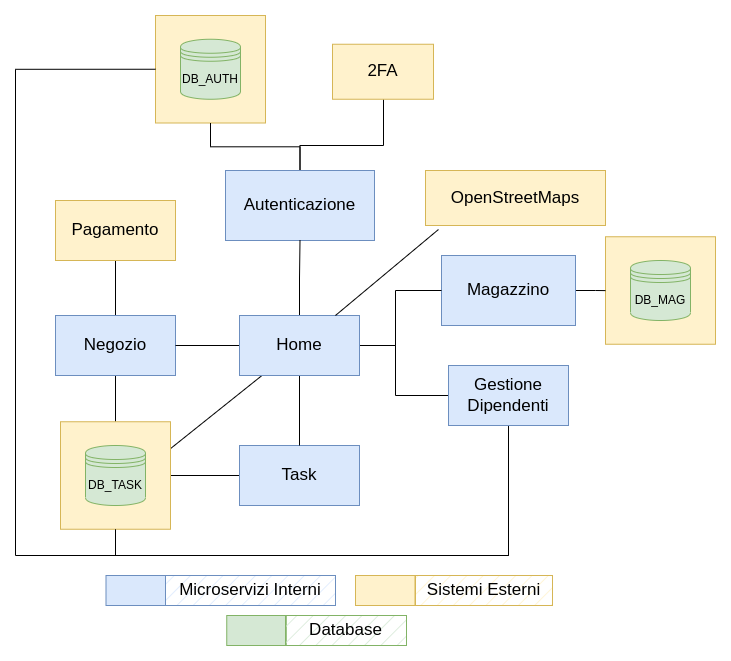
\includegraphics[width=0.6\textwidth]{back_end_short}
	\caption{Microservizi disponibili per tutti}
\end{figure}	

\begin{figure}[h]
	\centering
	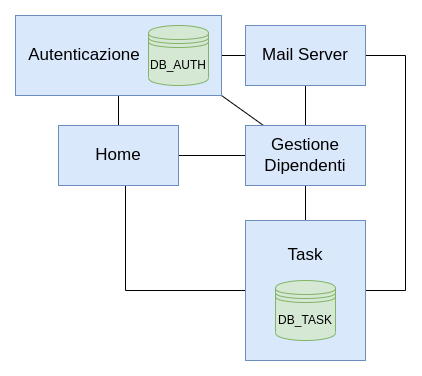
\includegraphics[width=0.4\textwidth]{admin_back_end}
	\caption{Gestione Dipendenti, disponibile solo per il manager}
\end{figure}

\begin{figure}[h]
	\centering
	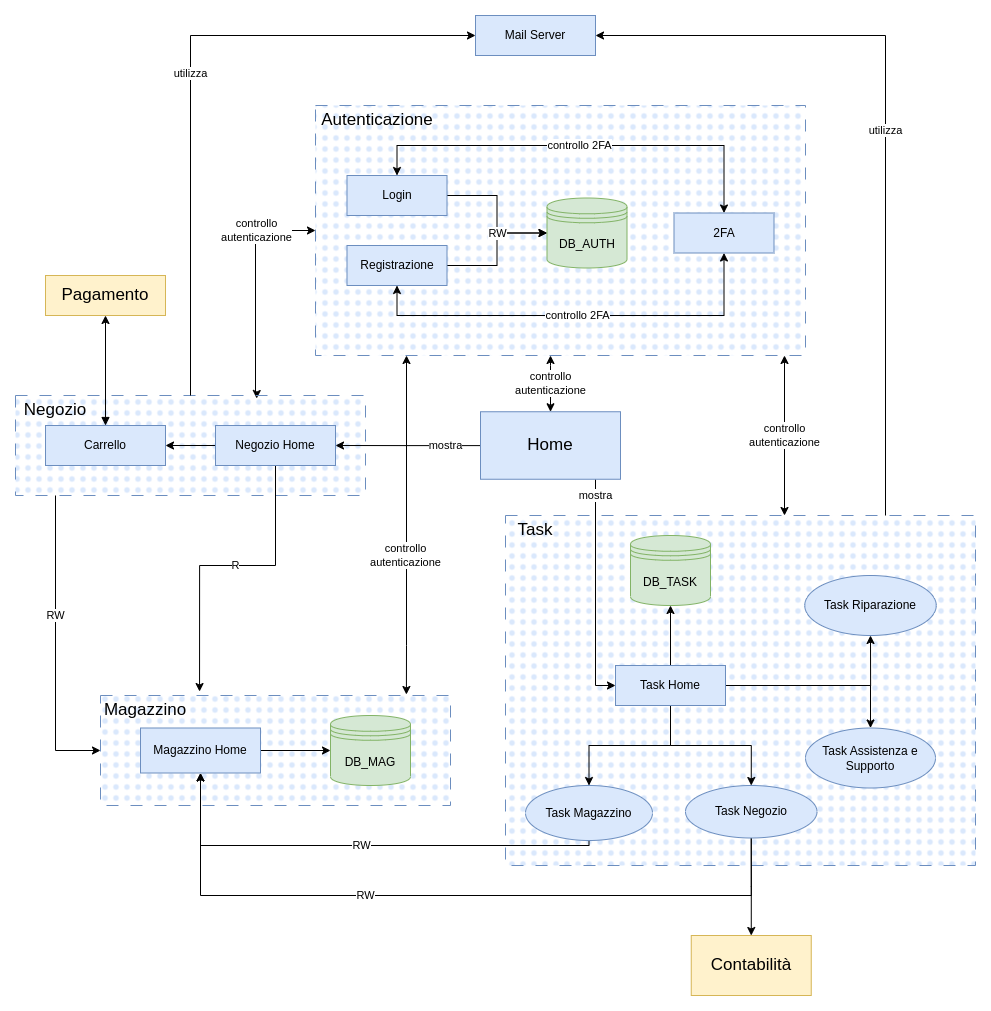
\includegraphics[width=1.1\textwidth]{backend_D1}
	\caption{Microservizi disponibili per tutti, con maggiore dettaglio}
\end{figure}



% -----------------------------

\chapter{Ruoli e Responsabilità}
Il team di sviluppo ha suddiviso l’obiettivo del progetto in obiettivi secondari di cui sono stati successivamente individuati ruoli e responsabilità:

% table
\begin{table}[!ht]
	\begin{center} % center the table
		\centering
		\begin{tabular}{ |p{4cm}|p{4cm}|  }
			\hline
			\centering Ruolo & \qquad\qquad Membro \\ % I found no other way...
			\hline
			Sviluppo dell'obiettivo & Il gruppo di sviluppo \\
			\hline
			Leader del team di sviluppo & Riginel Ungureanu \\
			\hline
			Supervisore Back-End &
			Giovanni Santini \\
			\hline
			Supervisore Front-End & Valerio Asaro\\
			\hline
		\end{tabular}
		\caption{Relazione tra Ruoli e Membri}
	\end{center}
\end{table}


\chapter{Tecniche e Strumentazione}
Diversi strumenti e tecniche sono state scelte accuratamente in base alla situazione posta dall’obiettivo. Di seguito un elenco degli strumenti utilizzati per la realizzazione del progetto:

\begin{itemize}
	\item Trello \qquad \url{https://trello.com/}
	\item GitHub \qquad \url{https://github.com/}
	\item Google Suite \qquad \url{https://workspace.google.it/intl/it/}
	\item LaTeX \qquad \url{https://www.latex-project.org/}
	\item Photoshop \qquad \url{https://www.adobe.com/it/products/photoshop.html}
	\item VSCode \qquad \url{https://code.visualstudio.com/}
	\item Figma \qquad \url{https://www.figma.com/}
	\item Coolors \qquad \url{https://coolors.co/}
	\item Diagrams \qquad \url{https://app.diagrams.net/}
\end{itemize}

\end{document}